\section{Testing and Evaluation}

\subsection{Test Architecture: 485 Tests}

Nexa-net's test suite comprises 485 tests organized across five categories:

\begin{table}[h]
\centering
\begin{tabular}{@{}lrl@{}}
\toprule
Category & Count & Description \\
\midrule
Unit tests & 433 & Per-module function/method tests \\
Integration tests & 31 & Cross-module interaction tests \\
E2E scenario tests & 10 & Full workflow validation \\
HTTP E2E tests & 5 & REST API endpoint tests \\
Property-based tests & 6 & Invariant validation via proptest \\
\midrule
\textbf{Total} & \textbf{485} & \\
\bottomrule
\end{tabular}
\caption{Test distribution across categories.}
\label{tab:test-distribution}
\end{table}

The test architecture follows the ``testing pyramid'' principle: a broad base of fast unit tests (433, $<$1ms each) validates individual functions; a middle layer of integration tests (31) validates cross-module interactions; and a narrow top of E2E tests (15) validates complete workflows. Property-based tests (6) supplement the pyramid by exploring edge cases that manual test design might miss.

\subsection{Unit Test Coverage}

Unit tests are organized per-module, covering each public function and error path:

\begin{itemize}
  \item \textbf{Identity} (src/identity/): DID generation, parsing, validation; DID Document creation, serialization; Ed25519 signing and verification; Verifiable Credential issuance and verification; Trust Anchor validation; KeyManagement store/get operations; mTLS certificate generation (design-level tests).
  \item \textbf{Discovery} (src/discovery/): CapabilitySchema registration, validation, serialization; Mock/ONNX vectorizer output consistency; HNSW index insertion, search, deletion; Kademlia routing table add-node, find-closest; SemanticRouter multi-factor scoring; NodeStatus update and health tracking.
  \item \textbf{Transport} (src/transport/): Frame header encode/decode; Stream state machine transitions; RPC message serialization; Negotiator protocol selection; Compression pipeline (JSON + LZ4/Zstd/Gzip); Error classification and retry logic.
  \item \textbf{Economy} (src/economy/): StateChannel creation, transfer, close; MicroReceipt generation, dual-signing, verification; Hash chain build and integrity check; BudgetController per-call/channel/agent limits; SettlementEngine balance computation; NexaToken issuance and transfer.
  \item \textbf{Security} (src/security/): SecureKeyStorage encrypt/decrypt; RateLimiter check and enforcement; AuditLogger append and chain verification; KeyRotator rotation lifecycle.
  \item \textbf{Storage} (src/storage/): MemoryStore CRUD operations; Cache set/get with TTL; Feature-gated backend trait compliance.
  \item \textbf{Proxy/API} (src/proxy/, src/api/): ProxyState initialization; REST handler request/response; NexaClient SDK builder and calls.
\end{itemize}

All unit tests run via \texttt{cargo test} in under 10 seconds, enabling rapid iteration during development. The tests verify both positive paths (correct input produces correct output) and negative paths (invalid input produces expected error types from the \texttt{NexaError} enum).

\subsection{Five E2E Scenarios}

The E2E tests validate complete agent-to-agent workflows through the proxy:

\textbf{Scenario 1: Dual-Agent Communication.} Two TestAgents (A and B) are created with distinct DIDs. Agent A registers a translation capability; Agent B discovers it via semantic search; a state channel is opened; an RPC call is made with a MicroReceipt; the channel is closed with settlement. This scenario validates the full data flow from intent to result.

\textbf{Scenario 2: Multi-Agent Community.} Five TestAgents form a community with diverse capabilities (translation, summarization, extraction). Each agent discovers and calls the others, creating a dense web of state channels. This scenario validates concurrent channel management and multi-factor routing under competitive selection.

\textbf{Scenario 3: Fault Recovery.} Agent A calls Agent B, but B's proxy crashes mid-RPC. The ErrorHandler detects the timeout, classifies it as transient, retries with exponential backoff, and eventually succeeds when B's proxy restarts. This scenario validates the error handling and retry strategy.

\textbf{Scenario 4: Economic Closed Loop.} Agent A deposits 100 NEXA into a channel with Agent B. A makes 10 calls to B, each generating a MicroReceipt with hash chain. The channel closes, and the SettlementEngine verifies all 10 receipts and computes final balances. This scenario validates the complete economic lifecycle: deposit $\rightarrow$ transfers $\rightarrow$ receipts $\rightarrow$ settlement.

\textbf{Scenario 5: Security Verification.} An attacker agent with an invalid DID attempts to register capabilities and open channels. The DID resolver rejects the invalid DID; the SecurityManager logs the attempt via AuditLogger; the RateLimiter blocks repeated attempts. This scenario validates the zero-trust security enforcement.

\subsection{HTTP E2E Testing with TestProxy}

The \texttt{TestProxy} infrastructure enables full HTTP-level E2E testing without external dependencies. TestProxy creates a real Axum server on a random port, initializes a ProxyState with test-friendly settings (min\_similarity = -1.0 to accept all matches), and provides a \texttt{reqwest} client for making actual HTTP requests.

The five HTTP E2E tests cover: (1) health endpoint returns 200 with valid JSON; (2) register endpoint accepts a valid capability and returns 201; (3) discover endpoint returns ranked results for a given intent; (4) duplicate registration is rejected with 409 Conflict; (5) discovery with no registered capabilities returns empty results. These tests validate that the REST API handlers work correctly with real HTTP transport, JSON serialization, and shared state access.

The TestProxy includes graceful shutdown logic: after the test completes, the server is shut down cleanly, releasing the bound port. The random port allocation (binding to port 0 and reading the assigned port) prevents port conflicts between concurrent test runs.

\subsection{Property-Based Testing with Proptest}

Proptest~\cite{proptest2019} generates random input combinations and validates structural invariants across thousands of iterations. Six proptest targets cover critical safety properties:

\begin{enumerate}
  \item \textbf{Balance invariant}: For any sequence of valid transfers in a state channel, $b_A + b_B = \text{total\_deposit}$ holds at every intermediate state. Proptest generates random transfer amounts and directions, confirming the invariant across 1000 iterations.

  \item \textbf{Receipt chain integrity}: For any sequence of MicroReceipts, the hash chain links correctly: $\text{receipt}_{i+1}.\text{previous\_hash} = \text{SHA-256}(\text{receipt}_i)$. Proptest generates random receipt content and verifies chain consistency.

  \item \textbf{VC verification determinism}: A properly issued VC always passes verification; a tampered VC always fails. Proptest generates random credential fields and verifies that signature verification is deterministic and collision-resistant.

  \item \textbf{HNSW search recall}: For any set of indexed vectors, HNSW search returns at least one result whose cosine similarity exceeds the minimum threshold. Proptest generates random 384-dimensional vectors and validates search recall.

  \item \textbf{Frame encode/decode round-trip}: For any valid frame header values, encoding followed by decoding produces identical output. Proptest generates random magic/version/type/flags/stream\_id/length combinations.

  \item \textbf{Budget enforcement}: For any combination of per-call, per-channel, and per-agent budgets, no transfer can violate any budget constraint. Proptest generates random budget configurations and transfer sequences.
\end{enumerate}

Proptest failures are recorded in \texttt{proptest-regressions/} files (e.g., \texttt{proptest-regressions/economy/channel.txt}, \texttt{proptest-regressions/identity/credential.txt}), enabling deterministic reproduction of any discovered edge case.

\begin{figure}[t]
\centering
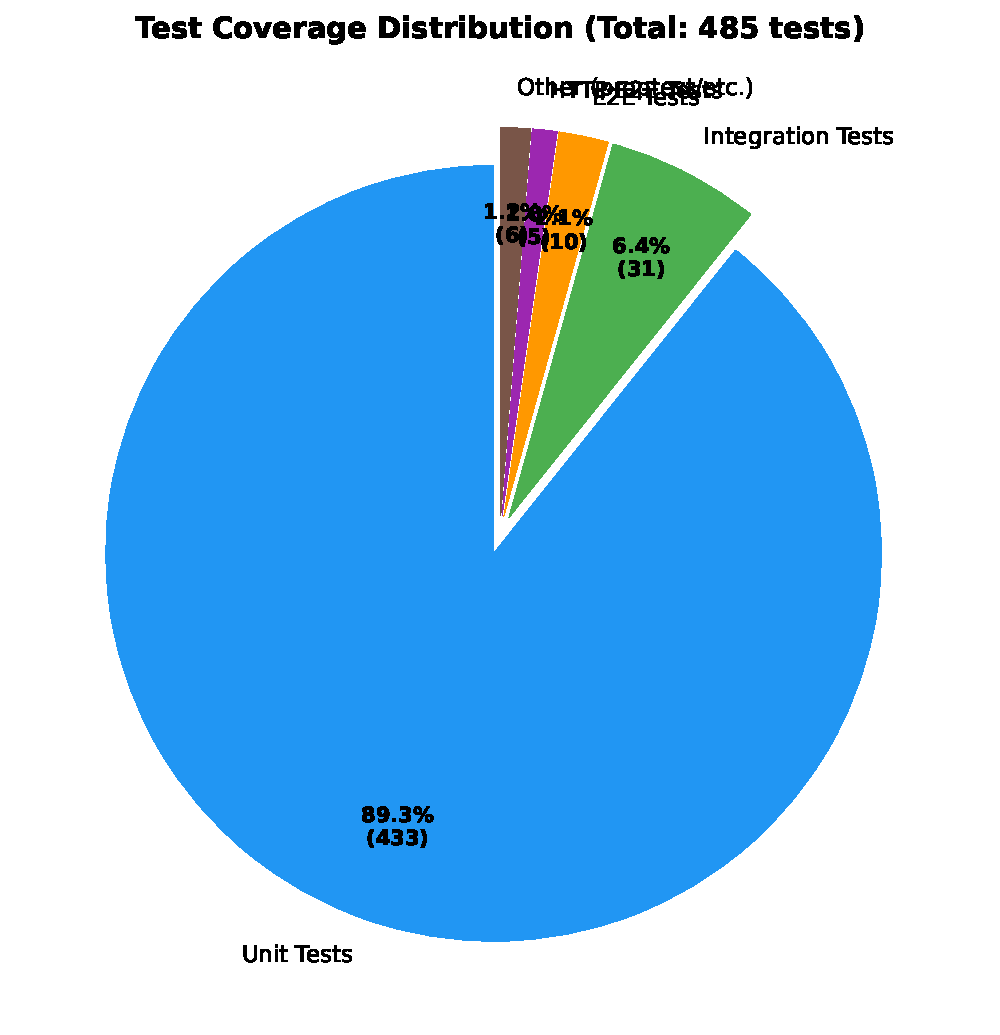
\includegraphics[width=0.7\columnwidth]{figures/test_coverage.pdf}
\caption{Test coverage distribution: 89.3\% unit tests, 6.4\% integration, 2.1\% E2E, 1.0\% HTTP E2E, 1.2\% property-based.}
\label{fig:test-coverage}
\end{figure}